% Classification trees (Section 6.2) --- from-zero deep-dive deck.
% Single tree (stuck bias) -> ensemble with Bayesian model averaging (bias drops).
% Standalone mini-deck, same metropolis style as ../presentation.tex.
% Build with: make   (tectonic)
\documentclass[aspectratio=169,10pt]{beamer}

\usetheme{metropolis}
\metroset{progressbar=frametitle, numbering=fraction, block=fill}

\usepackage[T1]{fontenc}
\usepackage{booktabs}
\usepackage{amsmath,amssymb}
\usepackage{tikz}
\usetikzlibrary{positioning,arrows.meta,fit,backgrounds,calc,matrix,decorations.pathreplacing}
\usepackage{xcolor}

% --- palette (identical to the main deck) ----------------------------------
\definecolor{accent}{HTML}{C1121F}
\definecolor{ink}{HTML}{2B2D42}
\definecolor{muted}{HTML}{6C757D}
\definecolor{good}{HTML}{2A9D8F}
\definecolor{biasc}{HTML}{2A6F97}
\setbeamercolor{frametitle}{bg=ink}
\setbeamercolor{background canvas}{bg=white}
\setbeamercolor{normal text}{fg=ink, bg=white}
\setbeamercolor{progress bar}{fg=accent}
\setbeamercolor{alerted text}{fg=accent}

\newcommand{\hl}[1]{{\color{accent}\textbf{#1}}}
\newcommand{\gd}[1]{{\color{good}\textbf{#1}}}
\newcommand{\mut}[1]{{\color{muted}#1}}
\newcommand{\cit}[1]{{\scriptsize\color{muted}[#1]}}

\title{Classification Trees as PFNs}
\subtitle{From one stuck tree to an ensemble that learns \;\cit{Nagler '23, \S6.2}}
\author{\underline{Gurmeher} Singh Puri \;\&\; Salih \underline{Bora} Öztürk}
\institute{Group 4 \;\textperiodcentered\; FM4SD Seminar \;\textperiodcentered\; SS26}
\date{}

\begin{document}

\maketitle

% ===========================================================================
% 1. What is a classification tree (from zero)
% ===========================================================================
\begin{frame}[t]{What is a classification tree? \mut{(from zero)}}

  \onslide<1->{\centering
    A tree \hl{chops feature space into regions} (``bins''), and to predict at $x$ it just reports
    the \hl{label mix} of whichever bin $x$ falls into.\par}
  \vspace{0.6em}

  \onslide<2->{\centering
    In 1-D this is simply \hl{cutting the number line} at split points $\theta_1<\theta_2<\dots$:\par}
  \vspace{0.3em}

  \onslide<2->{\centering
  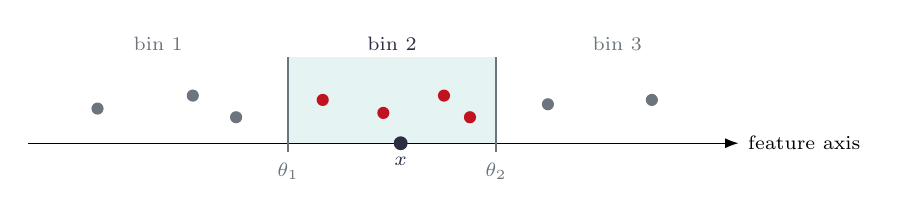
\begin{tikzpicture}[>=Latex, scale=1.1]
    \fill[good!12] (3.0,0) rectangle (5.4,1.0);
    \draw[->] (0,0) -- (8.2,0) node[right, font=\scriptsize]{feature axis};
    \foreach \tx/\lab in {3.0/$\theta_1$, 5.4/$\theta_2$}{
      \draw[muted, line width=0.6pt] (\tx,-0.1)--(\tx,1.0);
      \node[muted, font=\scriptsize, below] at (\tx,-0.12){\lab};}
    \node[muted, font=\scriptsize] at (1.5,1.15){bin 1};
    \node[ink, font=\scriptsize] at (4.2,1.15){bin 2};
    \node[muted, font=\scriptsize] at (6.8,1.15){bin 3};
    % points
    \foreach \p in {(0.8,0.4),(1.9,0.55),(2.4,0.3)} \fill[muted] \p circle(0.07);
    \foreach \p in {(3.4,0.5),(4.1,0.35),(4.8,0.55),(5.1,0.3)} \fill[accent] \p circle(0.07);
    \foreach \p in {(6.0,0.45),(7.2,0.5)} \fill[muted] \p circle(0.07);
    \fill[ink] (4.3,0) circle(0.08); \node[ink, font=\scriptsize, below] at (4.3,-0.05){$x$};
  \end{tikzpicture}}
  \vspace{0.5em}

  \onslide<3->{\centering
    $x$ lands in \gd{bin 2} $\Rightarrow$ look only at the points in bin 2 and report their label mix.\\[2pt]
    {\footnotesize\mut{(in 2-D the bins are rectangles; the idea is identical. The paper does 1-D for clarity.)}}\par}
\end{frame}

% ===========================================================================
% 2. Decode the formula
% ===========================================================================
\begin{frame}[t]{How it predicts --- decode the formula}

  \onslide<1->{\centering
  \[
    q_\theta(y\mid x,\mathcal D_n)=\sum_{j}\;
      \alt<2->{\textcolor{good!55!black}{\mathbf 1_{(\theta_j,\theta_{j+1}]}(x)}}{\textcolor{black!30}{\mathbf 1_{(\theta_j,\theta_{j+1}]}(x)}}\;
      \frac{\sum_i \alt<4->{\textcolor{accent}{\mathbf 1(Y_i=y)}}{\textcolor{black!30}{\mathbf 1(Y_i=y)}}\,
             \alt<3->{\textcolor{biasc}{\mathbf 1_{(\theta_j,\theta_{j+1}]}(X_i)}}{\textcolor{black!30}{\mathbf 1_{(\theta_j,\theta_{j+1}]}(X_i)}}}
           {\sum_i \alt<3->{\textcolor{biasc}{\mathbf 1_{(\theta_j,\theta_{j+1}]}(X_i)}}{\textcolor{black!30}{\mathbf 1_{(\theta_j,\theta_{j+1}]}(X_i)}}}
  \]\par}
  \vspace{0.5em}

  {\footnotesize
  \onslide<2->{$\bullet$\;\; {\color{good!55!black}$\mathbf 1_{(\theta_j,\theta_{j+1}]}(x)$} --- ``\textbf{which bin is $x$ in}'': this picks out the \emph{one} bin containing $x$ (all other terms vanish).\par}\smallskip
  \onslide<3->{$\bullet$\;\; {\color{biasc}$\mathbf 1_{(\theta_j,\theta_{j+1}]}(X_i)$} --- keep only the \textbf{training points in that bin} (denominator counts them).\par}\smallskip
  \onslide<4->{$\bullet$\;\; {\color{accent}$\mathbf 1(Y_i=y)$} --- of those, how many carry label $y$. So $q_\theta=\dfrac{\#\{\text{in bin \& label }y\}}{\#\{\text{in bin}\}}$ --- the bin's label fraction.\par}}
  \vspace{0.6em}

  \onslide<5->{\centering
    {\gd{Same shape as the window smoother}} --- a local average --- but the region is a \hl{fixed bin}, not a circle that follows $x$.\\[2pt]
    {\footnotesize\mut{The split points $\theta_1,\dots,\theta_S$ are the \hl{hyperparameters}, tuned \emph{offline} on prior datasets.}}\par}
\end{frame}

% ===========================================================================
% 3. Variance is fine
% ===========================================================================
\begin{frame}[t]{Variance: not a problem}

  \onslide<1->{\centering
    A tree is a \hl{local average}, so the same generic-smoother lemma applies \cit{Lem.\ 6.1}:
    each bin holds a roughly $n^{-\eta}$ share of the data, giving sensitivity exponent
    \hl{$\alpha=1$}.\par}
  \vspace{0.8em}

  \onslide<2->{\centering
    $\Rightarrow$ swap one sample, the bin's fraction barely moves $\Rightarrow$
    \gd{variance $\to 0$} as $n$ grows \cit{Thm 5.2}. \;Free, like everywhere else.\par}
  \vspace{0.8em}

  \onslide<3->{\centering
    {\footnotesize\mut{So, exactly as with the window smoother, the whole story is about \hl{bias}.}}\par}
\end{frame}

% ===========================================================================
% 4. The problem: bias is stuck
% ===========================================================================
\begin{frame}[t]{The problem: the bias is \emph{stuck}}

  \onslide<1->{\centering
    \[
      \text{bias}=\underbrace{\Pr_0\!\big(Y=y\mid X\in\text{bin}\big)}_{\text{true label-rate over the whole bin}}
      \;-\;\underbrace{p_0(y\mid x)}_{\text{true rate exactly at }x}.
    \]\par}
  \vspace{0.3em}

  \onslide<2->{\centering
    The split points are \hl{frozen}, so the bins never move. Adding data just fills the \emph{same}
    bins with more points.\par}
  \vspace{0.5em}

  \onslide<3->{\centering
  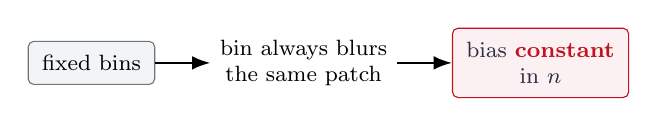
\begin{tikzpicture}[>=Latex, font=\footnotesize]
    \node[draw=muted, rounded corners=2pt, fill=muted!8, inner sep=5pt, align=center] (a) {fixed bins};
    \node[right=7mm of a, align=center] (b) {bin always blurs\\ the same patch};
    \node[draw=accent, rounded corners=2pt, fill=accent!6, inner sep=5pt, right=7mm of b, align=center, text=ink] (c)
      {bias \hl{constant}\\ in $n$};
    \draw[->, line width=0.8pt] (a)--(b); \draw[->, line width=0.8pt] (b)--(c);
  \end{tikzpicture}\par}
  \vspace{0.5em}

  \onslide<4->{\centering
    {\footnotesize\gd{Same disease as the fixed-window smoother:}} a \hl{fixed region $=$ fixed blur $=$ frozen bias}.
    More data $\Rightarrow$ tighter, not truer.\par}
\end{frame}

% ===========================================================================
% 5. Why we can't just fix one tree
% ===========================================================================
\begin{frame}[t]{Why we can't just sharpen the tree}

  \onslide<1->{\centering
    To shrink the blur you'd \hl{add more split points $S$} as $n$ grows --- finer bins, each closer to
    a single point, less blur. \mut{(Just like shrinking the window's radius.)}\par}
  \vspace{0.7em}

  \onslide<2->{\centering
  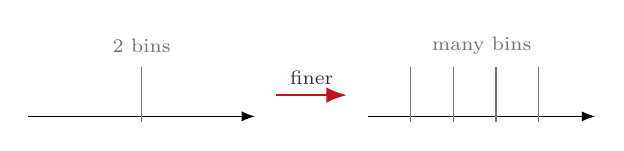
\begin{tikzpicture}[>=Latex, scale=0.9]
    % coarse
    \begin{scope}
      \draw[->] (0,0)--(3.2,0); \draw[muted](1.6,-0.08)--(1.6,0.7);
      \node[font=\scriptsize, muted] at (1.6,1.0){2 bins};
    \end{scope}
    \draw[->,line width=1pt,accent] (3.5,0.3)--(4.5,0.3) node[midway,above,font=\scriptsize,text=ink]{finer};
    % fine
    \begin{scope}[shift={(4.8,0)}]
      \draw[->] (0,0)--(3.2,0);
      \foreach \tx in {0.6,1.2,1.8,2.4} \draw[muted](\tx,-0.08)--(\tx,0.7);
      \node[font=\scriptsize, muted] at (1.6,1.0){many bins};
    \end{scope}
  \end{tikzpicture}}
  \vspace{0.8em}

  \onslide<3->{\centering
    But $S$ is a \hl{parameter}, and a PFN is \hl{frozen at inference} --- one forward pass, no new
    parameters. \;{\gd{You cannot grow the tree.}}\par}
  \vspace{0.3em}
  \onslide<4->{\centering
    {\footnotesize\mut{A single tree is therefore stuck. We need a fix that adds \emph{no} new parameters.}}\par}
\end{frame}

% ===========================================================================
% 6. The fix idea: many trees, vote
% ===========================================================================
\begin{frame}[t]{The fix: don't sharpen one tree --- \emph{vote} among many}

  \onslide<1->{\centering
    Keep a whole \hl{committee} of $K$ trees, all \emph{frozen}, each with \emph{different} split locations
    --- some coarse, some fine, splitting in different places.\par}
  \vspace{0.7em}

  \onslide<2->{\centering
  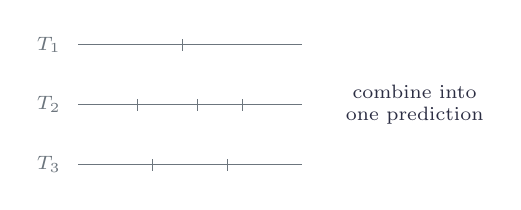
\begin{tikzpicture}[>=Latex, scale=0.95, font=\scriptsize]
    % T1 (coarse)
    \draw[muted] (0,1.6)--(3.0,1.6); \node[muted, left] at (-0.1,1.6){$T_1$};
    \draw[muted] (1.4,1.52)--(1.4,1.68);
    % T2 (fine)
    \draw[muted] (0,0.8)--(3.0,0.8); \node[muted, left] at (-0.1,0.8){$T_2$};
    \foreach \s in {0.8,1.6,2.2} \draw[muted] (\s,0.72)--(\s,0.88);
    % T3 (medium)
    \draw[muted] (0,0.0)--(3.0,0.0); \node[muted, left] at (-0.1,0.0){$T_3$};
    \foreach \s in {1.0,2.0} \draw[muted] (\s,-0.08)--(\s,0.08);
    \node[align=center, text=ink] at (4.5,0.8) {combine into\\ one prediction};
  \end{tikzpicture}}
  \vspace{0.8em}

  \onslide<3->{\centering
    Combine them into a single answer:
    \;$\displaystyle q_\theta(y\mid x,\mathcal D_n)=\sum_{k=1}^K w_k\, q_{\theta_k}(y\mid x,\mathcal D_n)$,\;
    a \hl{weighted average} of the trees.\par}
  \vspace{0.3em}
  \onslide<4->{\centering
    {\footnotesize\mut{The trees never change. The only question is: \hl{how do we set the weights $w_k$?}}}\par}
\end{frame}

% ===========================================================================
% 7. BMA + BIC
% ===========================================================================
\begin{frame}[t]{Weight each tree by how well it fits \mut{(Bayesian model averaging)}}

  \onslide<1->{\centering
    Give more say to the trees that \hl{explain the data better}:
    \[
      w_k=\frac{\exp\{-\mathrm{BIC}_k\}}{\sum_{j}\exp\{-\mathrm{BIC}_j\}}
      \qquad\mut{(\text{the }w_k\ge0\text{ sum to }1).}
    \]\par}
  \vspace{0.4em}

  \onslide<2->{\centering
    where \;$\displaystyle \mathrm{BIC}_k=\underbrace{-2\sum_{i}\log q_{\theta_k}(Y_i\mid X_i)}_{\textstyle\color{biasc}\text{how badly tree }k\text{ fits}}
      \;+\;\underbrace{S\log n}_{\textstyle\color{accent}\text{complexity penalty}}.$\par}
  \vspace{0.6em}

  \onslide<3->{\centering
    {\footnotesize
    {\color{biasc}fit term}: smaller when the tree puts high probability on the \emph{correct} labels.\quad
    {\color{accent}penalty}: charges for using more splits $S$ --- guards against overfitting.}\par}
  \vspace{0.3em}
  \onslide<4->{\centering
    \hl{Lower BIC $=$ better fit for its complexity}; \;$\exp\{-\mathrm{BIC}\}$ turns that into a weight.\par}
\end{frame}

% ===========================================================================
% 8. Why the ensemble learns
% ===========================================================================
\begin{frame}[t]{Why the ensemble \emph{learns} (bias drops with $n$)}

  \begin{columns}[T]
    \column{0.48\textwidth}
      \onslide<1->{\centering \textbf{small $n$}\\[4pt]
      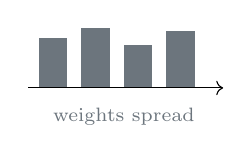
\begin{tikzpicture}[scale=0.9]
        \foreach \i/\h in {0/0.7,1/0.85,2/0.6,3/0.8}
          \fill[muted] (\i*0.6,0) rectangle (\i*0.6+0.4,\h);
        \draw[->](-0.15,0)--(2.6,0);
        \node[font=\scriptsize, muted] at (1.2,-0.4){weights spread};
      \end{tikzpicture}\\[2pt]
      {\footnotesize\mut{too little data to tell the trees apart.}}}
    \column{0.48\textwidth}
      \onslide<2->{\centering \textbf{large $n$}\\[4pt]
      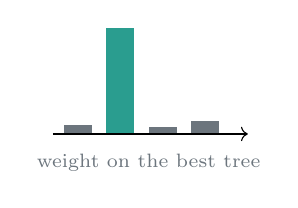
\begin{tikzpicture}[scale=0.9]
        \fill[muted] (0,0) rectangle (0.4,0.12);
        \fill[good]  (0.6,0) rectangle (1.0,1.5);
        \fill[muted] (1.2,0) rectangle (1.6,0.1);
        \fill[muted] (1.8,0) rectangle (2.2,0.18);
        \draw[->](-0.15,0)--(2.6,0);
        \node[font=\scriptsize, muted] at (1.2,-0.4){weight on the best tree};
      \end{tikzpicture}\\[2pt]
      {\footnotesize\gd{the data clearly favours the best fit.}}}
  \end{columns}
  \vspace{0.8em}

  \onslide<3->{\centering
    As $n$ grows the weights \hl{concentrate on the best-fitting trees}, so the ensemble drifts toward
    its strongest members $\Rightarrow$ \gd{the bias decreases} toward the best member's bias.\par}
  \vspace{0.4em}

  \onslide<4->{\centering
    {\footnotesize\hl{The key:} no parameter changed --- the trees stay frozen. The \emph{data-dependent weights}
    $w_k(\mathcal D_n)$ do the learning, and weights are allowed to depend on $\mathcal D_n$ at inference.}\par}
\end{frame}

% ===========================================================================
% 9. The big idea: implicit model selection
% ===========================================================================
\begin{frame}[t]{The big idea: implicit model selection}

  \onslide<1->{\centering
    The ensemble effectively \hl{picks the right sub-model} as evidence accumulates ---
    coarse trees early, finer trees once the data can justify them.\par}
  \vspace{0.8em}

  \onslide<2->{\centering
  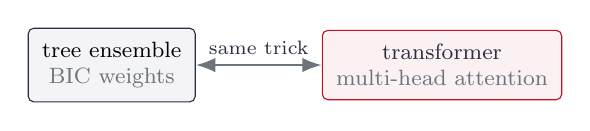
\begin{tikzpicture}[>=Latex, font=\footnotesize, node distance=6mm]
    \node[draw=ink, rounded corners=2pt, fill=ink!5, inner sep=5pt, align=center] (tree)
      {tree ensemble\\ \mut{BIC weights}};
    \node[right=16mm of tree, draw=accent, rounded corners=2pt, fill=accent!6, inner sep=5pt, align=center, text=ink] (tf)
      {transformer\\ \mut{multi-head attention}};
    \draw[<->, line width=0.9pt, muted] (tree)--(tf) node[midway, above, font=\scriptsize, text=ink]{same trick};
  \end{tikzpicture}}
  \vspace{0.8em}

  \onslide<3->{\centering
    A transformer does the \emph{same} thing with \hl{multiple attention heads}: different heads $=$ different
    sub-models, blended by the network. \;$H>1$ is what lets TabPFN's bias fall --- up to its trained sizes.\par}
  \vspace{0.3em}
  \onslide<4->{\centering
    {\footnotesize\mut{So the toy tree-ensemble is a clean window into \emph{why} a real PFN can reduce bias at all.}}\par}
\end{frame}

% ===========================================================================
% 10. Summary
% ===========================================================================
\begin{frame}[t]{Summary}

  \onslide<1->{\centering
  \renewcommand{\arraystretch}{1.3}
  \begin{tabular}{@{}lcc@{}}
    \toprule
    & \textbf{Variance} & \textbf{Bias as $n\!\uparrow$} \\
    \midrule
    Single frozen tree                  & $\to 0$ & \hl{stuck} \mut{(fixed bins)} \\
    Ensemble $+$ model averaging        & $\to 0$ & \gd{decreases} \mut{(best tree wins)} \\
    \bottomrule
  \end{tabular}\par}
  \vspace{1.0em}

  \onslide<2->{\begin{itemize}\setlength\itemsep{0.5em}
    \item A single tree is a local average over \hl{fixed bins} $\Rightarrow$ fixed blur $\Rightarrow$ \hl{frozen bias}.
    \item You can't add splits (frozen model), so instead \gd{average many trees, weighted by fit}.
    \item As $n$ grows the weights \gd{select the best trees} $\Rightarrow$ bias falls --- \emph{no new parameters}.
    \item Same mechanism as a transformer's \hl{multi-head attention}.
  \end{itemize}}
\end{frame}

% ===========================================================================
\begin{frame}[standout]
  One frozen tree is stuck.\\[6pt]
  A committee of trees, weighted by fit,\\
  \emph{selects} its best member as data grows --- so the bias falls.
\end{frame}

\end{document}
